\chapter{Modellierung von Patchwork als Computerprogramm}
\label{chapter:modellierung-von-patchwork-als-computerprogramm}

TODO: Erst generelle Architektur, Programmiersprache usw. hier auch generelle speicherung (spieler, Sonderplättchen, zeitplan, ...)

\begin{itemize}
    \item Aufbau des Spielfeldes
    \item Speicherung der Quilt Boards (Row-Major)
    \item Speicherung des Time Boards
    \item Speicherung der Patchliste
    \item Umsetzung von Zügen
    \item Effizienzoptimierungen (u128, vorberechnete Transformationen, ...)
    \item Abstraction von Player Interface
    \item Evaluator, Move Orderer, Tree Policy (wahrscheinlich später)
\end{itemize}

TODO: Zeitplan einfaches Array mit Bitflags

Besondere extra:

\section{Aufbau des Ablageplans}

TODO:

\begin{figure}[!ht]
    \centering
    \rlap{{\color{white}\acf{LSB} \acf{MSB}}} \vspace*{-\baselineskip}
    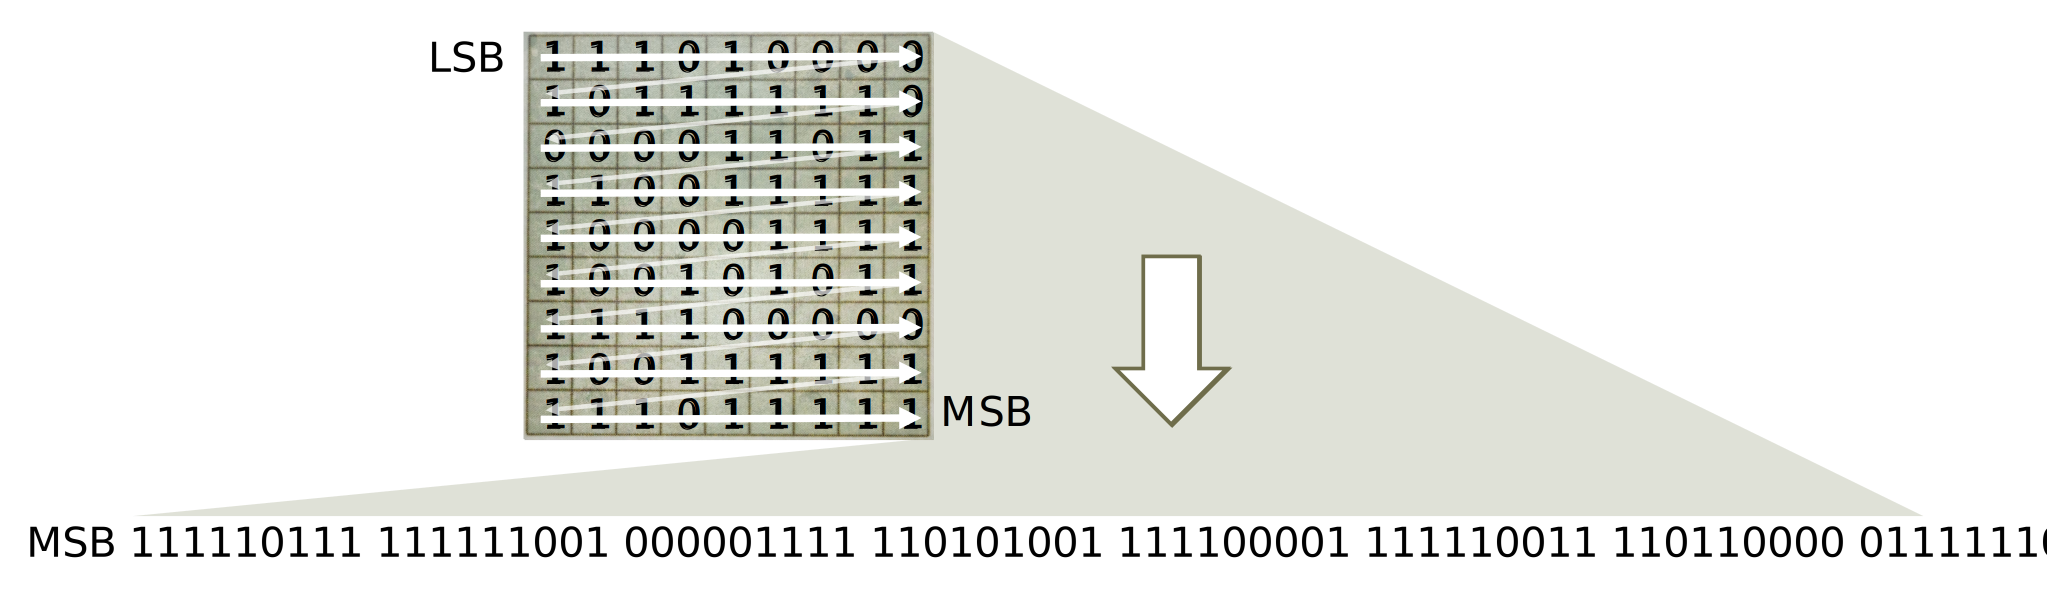
\includegraphics[width=\textwidth]{res/pictures/quilt-board-storage.pdf}
    \caption{Zeilenweise Anordnung der Felder des Ablageplans}
    \label{fig:quilt-board-storage}
\end{figure}

\section{Modellierung der Aktionen}

TODO: Action, ActionId/SurrogateActionId, NaturalActionId

\lstinputlisting[
    label={code:action},
    caption={Definition des Tagged-Union \code{Action}},
    captionpos=b,
    language=Rust,
    firstline=0,
]{res/code/action.rs}

\begin{itemize}
    \item \code{Action} als Tagged-Union
    \item \code{ActionId} bzw. \code{SurrogateActionId} als \ac{u32}
    \item \code{NaturalActionId} als TODO: 2028
\end{itemize}

\section{Flicken und Zugmöglichkeiten}

\acs{u128}

\pagebreak

\begin{table}[H]
    \centering
    \resizebox{\textwidth}{!}{\begin{tabular}{|l|r|c|l|}
            \hline
            \multicolumn{1}{|c|}{Methode}                                                 & \multicolumn{1}{|c|}{Zeit} & $\mathcal{O}$-Kalkül        & \multicolumn{1}{|c|}{Bemerkungen}                  \\ \hline
            \code{game.get\_initial\_state}                                               & $472{,}11\,\acs{ns}$       & $\mathcal{O}\left(n\right)$ & $n$ aufgrund Mischen der Flicken                   \\  \hline
            \code{game.get\_valid\_actions}                                               & $8{,}91\,\acs{us}$         & $\mathcal{O}\left(n\right)$ & $3\times$Aufruf von Ablageplan Aktionen generieren \\  \hline
            \code{game.get\_random\_action}                                               & $9{,}22\,\acs{us}$         & $\mathcal{O}\left(n\right)$ & Aufruf von \code{get\_valid\_actions}              \\  \hline
            \code{game.do\_action}                                                        & $280{,}00\,\acs{ns}$       & $\mathcal{O}\left(1\right)$ &                                                    \\  \hline
            \code{game.undo\_action}                                                      & $286{,}78\,\acs{ns}$       & $\mathcal{O}\left(1\right)$ &                                                    \\  \hline
            \code{game.clone}                                                             & $1{,}36\,\acs{us}$         & $\mathcal{O}\left(1\right)$ & $\hat{=}$ \code{memcpy}                            \\  \hline
            \code{game.is\_terminated}                                                    & $84{,}79\,\acs{ns}$        & $\mathcal{O}\left(1\right)$ &                                                    \\  \hline
            {\footnotesize \code{action\_id.from\_natural\_action\_id} }                  & $42{,}44\,\acs{ns}$        & $\mathcal{O}\left(1\right)$ &                                                    \\  \hline
            {\footnotesize \code{natural\_action\_id.from\_surrogate\_action\_id} }       & $45{,}97\,\acs{ns}$        & $\mathcal{O}\left(1\right)$ &                                                    \\  \hline
            \code{patch\_manager.get\_patch}                                              & $1{,}87\,\acs{ns}$         & $\mathcal{O}\left(1\right)$ &                                                    \\  \hline
            \code{patch\_manager.get\_special\_patch}                                     & $3{,}70\,\acs{ns}$         & $\mathcal{O}\left(1\right)$ &                                                    \\  \hline
            \code{patch\_manager.get\_transformation}                                     & $2{,}57\,\acs{ns}$         & $\mathcal{O}\left(1\right)$ &                                                    \\  \hline
            \code{player.get\_position}                                                   & $41{,}93\,\acs{ns}$        & $\mathcal{O}\left(1\right)$ &                                                    \\  \hline
            \code{quilt\_board.is\_full}                                                  & $561{,}16\,\acs{ps}$       & $\mathcal{O}\left(1\right)$ &                                                    \\  \hline
            {\footnotesize \code{quilt\_board.is\_special\_tile\_condition\_reached} }    & $523{,}76\,\acs{ps}$       & $\mathcal{O}\left(1\right)$ &                                                    \\  \hline
            \code{quilt\_board.do\_action}                                                & $46{,}90\,\acs{ns}$        & $\mathcal{O}\left(1\right)$ &                                                    \\  \hline
            \code{quilt\_board.undo\_action}                                              & $47{,}18\,\acs{ns}$        & $\mathcal{O}\left(1\right)$ &                                                    \\  \hline
            {\footnotesize \code{quilt\_board.get\_valid\_actions\_for\_patch} }          & $1{,}27\,\acs{us}$         & $\mathcal{O}\left(n\right)$ &                                                    \\  \hline
            {\footnotesize \code{quilt\_board.get\_valid\_actions\_for\_special\_patch} } & $855{,}98\,\acs{ns}$       & $\mathcal{O}\left(n\right)$ &                                                    \\  \hline
            Getter\textendash{} und Setter\textendash{}Methoden                           & $\diagup$                  & $\mathcal{O}\left(1\right)$ &                                                    \\  \hline
        \end{tabular}}
    \vspace{3pt}
    \caption{Übersicht über die verfügbaren Methoden in der Patchwork\textendash{}Implementierung}
    \label{tabelle:patchwork-methods}
\end{table}

TODO: Hier fehlt noch der Anhang + Verweis für Benchmark